\documentclass[./../../paper.tex]{subfiles}
\graphicspath{{\subfix{./../../figures/}}}

\begin{document}

\section{Choosing the Prediction and Feasibility Model}
Before testing any model we have to establish two crucial components of the viability measure. First, we require a prediction model which we want to explain using counterfactuals. This is relevant for determining the improvement that a counterfactual yileds in contrast to the factual. Second, we need to know to what extend any given counterfacual is feasbile given the dataset at hand. Therefore, we will dedicate the first set of experiments to establishing these components.

\subsection{Prediction Model}
We use counterfactuals primarily to explain predictive models. This explanation requires a to define the prediction model we use in this thesis.

\subsubsection{Model Description}
As explained in \autoref{sec:lstm_prediction_model}, we use a \gls{LSTM}.
The architecture of the model is shown in \autoref{fig:lstm_architecture}.

One input consists of an 2-dimensional event tensor containing integers. The second input is a 3-dimensional tensor containing the remaining feature attributes. The first dimension in each layer represents the variable batch size and \emph{None} acts as a placeholder.

The next layer is primarily concerned with preparing the full vector representation. We encode each activity in the sequence into a vector-space. We chose a dense-vector representation instead of a one-hot representation. We also create positional embeddings. Then we concat the activity embedding, positional embedding and the event attribute representation to a final vector representation for the event that occured.

Afterwards, we pass the tensor through a \gls{LSTM} module. We use the output of the last step to predict the outcome of a sequence using a fully connected neural network layer with a sigmoid activation as this is a binary classification task.

\begin{figure}[hpb]
    \centering
    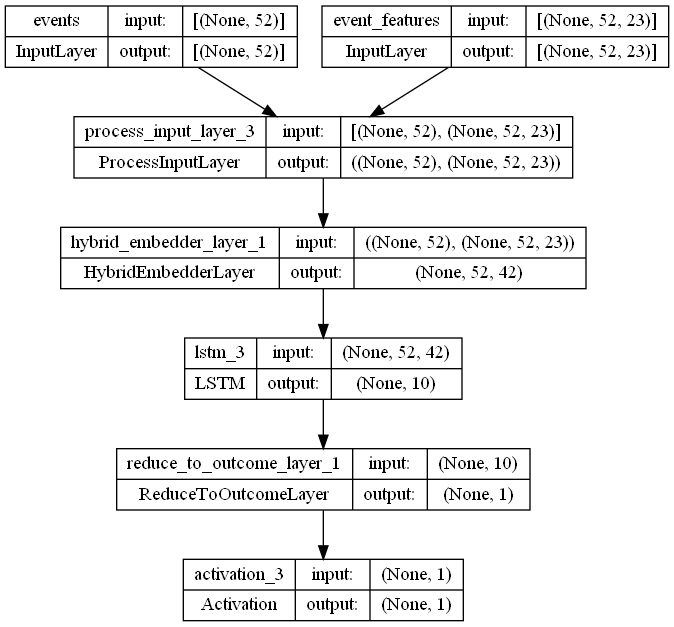
\includegraphics[width=0.8\textwidth]{figures/predictor50lstm.png}
    \caption{Shows the different components of the LSTM architecture. Each elements contains information about the input and output of a layer. None is a placeholder for the batch size.}
    \label{fig:lstm_architecture}
\end{figure}

\subsubsection{Practical Matters}
\attention{Mention everything necessary to repeat this experiment: For instance, unbalanced data}

\subsubsection{Results}
\attention{Show how this model is fine to use by reporting training and validation scores.}

\subsubsection{Discussion}
\optional{Mention whatever is noticable: 1. The models are extremely good for longer maximal sequence lengths of the BPIC dataset. The question is whether the model genuinely learns intrinsic features or just waits for trivial patterns like: How many padding events does the sequence have? What cyclical patterns are present? Does a particular event occur or not. Could be solved using attention and a visualisation method.}


\subsection{Feasibility Model}
To compute the viability of a counterfactual we need to determine its feasibility. In other words, we have to determine the possibility or impossibility of the counterfactual. We can use the data log to gauge the feasibility, by estimating the data distribution.

There are many ways to estimate the density of a data set. For our purposes, we incorporate the sequential structure of the log data and make simplifying assumptions. First, we consider every activity as a state in the case. Second, each state is only dependent on its immediate predecessor and neither on future nor on any any states prior to its immediate predecessor. Third, the collection of attributes within an event depend on the activity which emits it. The second assumption is commonly known as \emph{Markov Assumption}. With these assumptions in place, we can model the distribution by knowing the state transition probability and the density to emit a collection of event attributes given the activity. The probability distributions are shown in \autoref{eq:feasibility_model}.


\begin{figure}[htbp]
    \centering
    \begin{tikzpicture}[->,>=stealth',auto,semithick,node distance=2cm]
        % \tikzstyle{every state}=[fill=white,draw=black,thick,text=black,scale=1]
        % https://aditya-sengupta.github.io/expository/markovtex.pdf
        % https://tex.stackexchange.com/a/89663
        \node[circle, draw] (t0) {$e_{0}$};
        \node[circle, draw] (t1) [right of=t0] {$e_{1}$};
        \node[circle, draw] (t2) [right of=t1] {$e_{2}$};
        \node[circle, draw] (tn) [right=of t2] {\ldots};
        \node[circle, draw] (tN) [right=of tn] {$e_{T}$};
        \node[circle, draw] (f0) [below of=t0] {$f_0$};
        \node[circle, draw] (f1) [below of=t1] {$f_1$};
        \node[circle, draw] (f2) [below of=t2] {$f_2$};
        \node[circle, draw] (fT) [below of=tN] {$f_T$};
        % \node[draw=none] (tn) [right=of t2] {\ldots};
        \path (t0) edge (t1);
        \path (t1) edge (t2);
        \path (t1) edge (t2);
        \path (t2) edge (tn);
        \path (tn) edge (tN);
        \path (t0) edge (f0);
        \path (t1) edge (f1);
        \path (t2) edge (f2);
        \path (tN) edge (fT);

    \end{tikzpicture}
    \caption{The feaibility model in graphical form.}
    \label{fig:markov_model}
\end{figure}

% \needsequation{eq:feasibility_model}

% \begin{figure}[htbp]
    \centering
    \begin{tikzpicture}[->,>=stealth',auto,semithick,node distance=2cm]
        % \tikzstyle{every state}=[fill=white,draw=black,thick,text=black,scale=1]
        % https://aditya-sengupta.github.io/expository/markovtex.pdf
        % https://tex.stackexchange.com/a/89663
        \node[circle, draw] (t0) {$e_{0}$};
        \node[circle, draw] (t1) [right of=t0] {$e_{1}$};
        \node[circle, draw] (t2) [right of=t1] {$e_{2}$};
        \node[circle, draw] (tn) [right=of t2] {\ldots};
        \node[circle, draw] (tN) [right=of tn] {$e_{T}$};
        \node[circle, draw] (f0) [below of=t0] {$f_0$};
        \node[circle, draw] (f1) [below of=t1] {$f_1$};
        \node[circle, draw] (f2) [below of=t2] {$f_2$};
        \node[circle, draw] (fT) [below of=tN] {$f_T$};
        % \node[draw=none] (tn) [right=of t2] {\ldots};
        \path (t0) edge (t1);
        \path (t1) edge (t2);
        \path (t1) edge (t2);
        \path (t2) edge (tn);
        \path (tn) edge (tN);
        \path (t0) edge (f0);
        \path (t1) edge (f1);
        \path (t2) edge (f2);
        \path (tN) edge (fT);

    \end{tikzpicture}
    \caption{The feaibility model in graphical form. $e_t$ represents an event and $f_t$ the features it emits.}
    \label{fig:markov_model}
\end{figure}


\noindent Here, $e_t$ represents the transition from one event state to another. Likewise, $f$ represent the emission of the feature attributes.  Hence, the probability of a particular sequence is the product of the transition probability multiplied with state emission probability for each step. Note, that this is the same as the feasibility measure as in \autoref{eq:feasibility_measure}. \attention{Make formula in viability section consistent with this! Formula needs to use e instead of a and change starting index from 1 to 0.}

\begin{align}
    \prob{e_{0:T},f_{0:T}} & = \prob{e_0}\cprob{f_0}{e_0}\prod_1^T \cprob{e_t}{e_{t-1}} \cprob{f_t}{e_t}
\end{align}


\subsubsection{Practical Matters}
The general computation of these products is trivial. However, we need to probabilities for $\prob{e_0}$, $\cprob{f_t}{e_t}$ and $\cprob{e_t}{e_{t-1}}$ as the true distributions are unobservable.

Starting with the transition dynamics part of the equation $\cprob{e_t}{e_{t-1}}$, we can estimate the model parameters by counting the transitions from one event state \optional{(acitvity)} to another \optional{(acitvity)}.\attention{Define the difference between event und activity in a better way and earlier.} $\prob{e_0}$ is a special case, as it does not have a preceding event.

The emission probabilities are more complicated for three reasons: First, the event distribution does not necessarily belong to the same family as the feature distribution. Hence, we cannot use any simple method to estimate these conditionals. We need to estimate the probability for each event seperately. \xixi{Should I change this to density function instead. AFAIK mathematicians distinguish between density functions and probability functions. They often reserve \emph{probability} for discrete probability functions and \emph{density} for continous probability functions.}

The second issue directly follows from the first. If we estimate each event distribution by partioning the data by events, we naturally have less data to estimate each model's parameters. Although, event partitioning, are not an issue for common events states \optional{(activities)}, they can make emission probabilities of less frequent event states exceptionally hard to estimate.
One can turn to Bayesian Methods, which hand these situations better by specifying a prior.

However, the third issue exacerbates the main issue of using bayesian methods. Namely, because features do not necessarily have to be from the same distributional family, we have to model each conditional distribution with a mixture of distributions. Hence, simple bayesian updates are not possible either \optional{and require more time expensive methods such as Markov-Chain-Monte-Carlo methods or similar}.\attention{Check if this is true. Maybe we \emph{can} use MCSC}.

From these issues, we can conclude there are multiple viable ways to model these conditional distributions and we have to choose an fitting method\footnotemark. \footnotetext{Note, that we did not mention modelling $\cprob{f_0}{e_0}$ as it is practically the same distribution as $\cprob{f_t}{e_t}$.}

\subsubsection{Model Description}
Knowing, there are many ways to model the sequence distribution, we choose to implement a number of different menthods. However, we evaluate them based on how well they fit the data distribution and choose the most promising method.

\noindent\textbf{Transition Dynamics:} For the transition dynamics we count the individual transitions as mentioned by using a \emph{Transition-Count-Matrix}. Then, we compute the probabilities of each transition by dividing occurence count of the preceding event-state. We apply the same method on the $\prob{e_0}$. The only difference is that we count the starts and divide by thenumber of available cases.

\noindent\textbf{Emission Probability:} For $\cprob{f_t}{e_t}$, we employ \attention{3} tactics:
\begin{enumerate}
    \item[Independent:] Here, we assume all feature columns are independent variables with no covariations. Hence, for discrete variables, we use Categorical distributions. In other words, if the variable is binary, we count the ones to estimate the parameters of a Bernoulli distribution. Similar holds for categorical distributions. In contrast, we use independent Gaussian distributions for continuous variables.
    \item[Grouped:] Here, we group variables from the same distributional family and estimate their parameters. Meaning, we take all discrete distributions and compute the parameters of one categorical distribution. Likewise, we group all continuous variables and compute the parameters, mean and covariance, for one multivariate Gaussian distribution.
    \item[Grouped with $\chi^2$:] This is similar to the grouped approach. However, a multivariate Gaussian is also a continuous distribution. The likelihood of a continuous density distribution is not limited to a range between 0 and 1. Only the area under the density funtion has to follow this restriction. Meaning, if we compute the likelihood of a specific data point we might end up values of 30 or event 300000. Therefore, we rather interprete a data point as the mean of a another Gaussian. With this assumption, we can use the $\chi^2$ distribution to compute the probability of that distribution belonging to the distribution at hand. Or rather, how likely it is to find another datapoint which is more likely to belong to the distribution. Here, we say $Q=(Y-\mu)^{T} \Sigma^{-1}(Y-\mu)$  and assume $Q \sim \chi^{2}(k)$. If Q is bigger than $(x-\mu)^{T} \Sigma^{-1}(x-\mu)$, then $\mathbb{P}\left[(y-\mu)^{T} \Sigma^{-1}(y-\mu) \geq(x-\mu)^{T} \Sigma^{-1}(x-\mu)\right]=1-\mathbb{P}\left[Q \leq(x-\mu)^{T} \Sigma^{-1}(x-\mu)\right]$
\end{enumerate}

\noindent\textbf{Gaussian Distribution under Event Partitions}
\xixi{This section requires an intuitive understanding of linear algebra and the formula of simple gaussians and multivariate gaussians. Shall I put this in the discussion section instead?}
Gaussian distributions are particularly vulnerable to data shortages due to event partionings.

For instance, if we use independent variables, we often face issues of columns without any variation. Those lead to a covariance matrices' determinant being 0. In these cases the covariance is no longer a definite covariance matrix. A determinant with a value of 0 means intuitively, that at least one of the Gaussian distributions has an undefined probability. This undefinable probability occurs, because the variance parameter of a regular Gaussian appears in the denominator of the whole expression. By dividing by 0 and subsequently computing the joint probability we receive an undefined joint probability. Therefore, the covariance often needs to be definite. This issue is the reason, why  we often employ numerical solutions like \emph{Singular-Value-Composition} to get an approximation.

However, if the covariance matrix has a higher rank than the number of data points used to estimate if, the issue remains. Meaning, if we have a 20x20 covariance matrix and just 3 datapoints to estimate it, we will likely face numerical issues of computing the determinant again.

To mitigate these issues, we fallback to methods like adding a small constant to the diagonal. If this approach does not work either, we add a small constant to the full matrix. Alternatively, we can compute the Gaussian in a Bayesian way by adding a prior. However, using a fallbacks was deemed as the simpler solution.

\subsubsection{Results}
With all the configurations in mind we compare the distribution of the dataset with the distribution drawn from samples from the distribution. The configuration which best represent the data distribution is the best candidate for the next experimental steps. For this purpose, compute we the feasibility values for the Log's cases for the whole training dataset. Additionally, we sample the same number of values using our distributional approach. We show their distributions in \autoref{fig:distributions}.


\begin{figure}
    \centering
    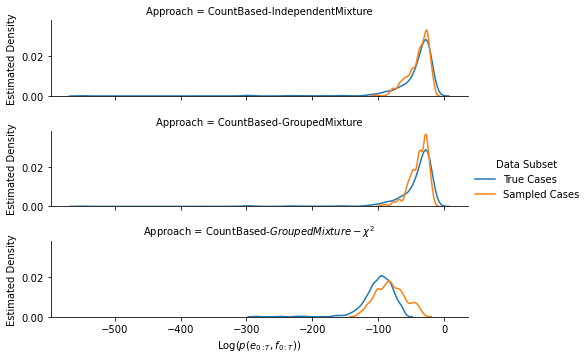
\includegraphics[width=\textwidth]{figures/results/result_distributions.png}
    \caption{The figure shows the distribution of feasibility values given the approach that was used. It is not entirely clear which of the approaches fit better to the data.}
    \label{fig:distributions}
\end{figure}

As the figure is difficult to interpret subjectively, we also compute various distances using the same subsets of data. The Kolgomorov-Smirnoff Test (KST) is particularly interesting as it is a common method to compute the difference between two distributions.

\begin{table}
    \caption{Table show the computation of various distances. Showing that the combination of Countbased Transition Estimation and the Gouped-$\chi^2$ approach consistently yields lower distances.}
    \label{tbl:distributions}
    \begin{tabular}{lllr}
     & Transition Approach & Emmision Approach & value \\
    Eval-Method &  &  &  \\
    KS-Test & CountBased & GroupedMixture & 0.411523 \\
    KS-Test & CountBased & GroupedMixture-$\chi^2$ & 0.353909 \\
    KS-Test & CountBased & IndependentMixture & 0.419753 \\
    L2 & CountBased & GroupedMixture & 0.000004 \\
    L2 & CountBased & GroupedMixture-$\chi^2$ & 0.000000 \\
    L2 & CountBased & IndependentMixture & 0.000004 \\
    L1 & CountBased & GroupedMixture & 0.000033 \\
    L1 & CountBased & GroupedMixture-$\chi^2$ & 0.000000 \\
    L1 & CountBased & IndependentMixture & 0.000031 \\
    Correlation & CountBased & GroupedMixture & 1.004166 \\
    Correlation & CountBased & GroupedMixture-$\chi^2$ & 1.004104 \\
    Correlation & CountBased & IndependentMixture & 1.010678 \\
    \end{tabular}
\end{table}

\autoref{tbl:distributions} shows that the third approach yields lower distances accross all distance methods employed.

\subsubsection{Discussion}
As the best configuration seems to be the \attention{CountBased-Grouped-$\chi^2$} approach, we continue with this configuration for the subsequent experiments.

However, it is important to stress that the proposed way of estimating the data distribution is one of many. The markovian approach explicitly removes the effect of past and future states. It is needless to say, a process step does not have to depend on its immediate previous state. A process outcome may be influenced by all past or future events. For instance, if one has to approve a loan in a second stage, one might be more inclined to approve something that a trusted employee already approved. Likewise, one might apply more scrutiny, knowing that a certain supervisor is going to approve the third stage.

Furthermore, this approach assumes strictly sequential processes. If the sequence has events running in parallel, we also have to record in greater detail which event has triggered a subsequent event in a given sequence. Often this knowledge is not even available.

\attention{Mention to Discuss issue with underflow}



\end{document}